\documentclass[11pt]{article}

\usepackage{amsmath}
\usepackage{booktabs}
\usepackage{braket}
\usepackage{chemfig}
\usepackage{chemformula}
\usepackage[outline]{contour}
\usepackage{enumitem}
\usepackage[T1]{fontenc}
\usepackage[margin=1in]{geometry}
\usepackage{graphicx}
\usepackage[utf8]{inputenc}
\usepackage{libertine}
\usepackage{mathtools}
\usepackage[libertine]{newtxmath}
\usepackage{pgfplots}
\usepackage[detect-weight=true]{siunitx}

\title{PHYS 234 Assignment 2}
\author{Brandon Tsang}
\date{May 29, 2020}

\pgfplotsset{compat=1.17}
\contourlength{0.1em}
\newcommand\uline[1]{\underline{\smash{#1}}\llap{\contour{white}{#1}}}
\DeclarePairedDelimiter\abs{\lvert}{\rvert}
\makeatletter
\let\oldabs\abs
\def\abs{\@ifstar{\oldabs}{\oldabs*}}
\let\oldnorm\norm
\def\norm{\@ifstar{\oldnorm}{\oldnorm*}}
\makeatother

\newenvironment{amatrix}[1]{%
    \left[\begin{array}{@{}*{#1}{c}|c@{}}
}{%
    \end{array}\right]
}

\begin{document}
    \maketitle
    \begin{enumerate}[label=\textbf{\arabic*.}, start=3]
        \item{
            \textbf{\boldmath \uline{Three Stern-Gerlach Analyzers with Arbitrary Direction} \\ A beam of spin-\(\frac 1 2\) particles is sent through a series of three S-G analyzers, as shown in the figure. The second S-G analyzer is aligned along the \(\hat{n}\)-direction. \begin{center}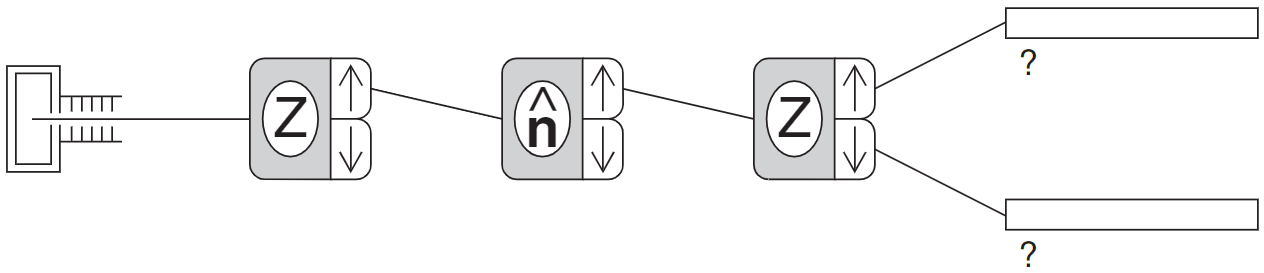
\includegraphics[width=5in]{235.PNG}\end{center}}
            \begin{enumerate}[label=\textbf{(\alph*)}]
                \item{
                    \textbf{Find the probability that particles transmitted through the first S-G analyzer are measured to have spin down at the third S-G analyzer.}
                    \par
                    This would be the probability of the particles going through the first two analyzers multiplied by the probability of those particles going through the third analyzer.
                    \begin{align*}
                        \abs{\braket{+|+}_n}^2\abs{\prescript{}{n}{\braket{+|-}}}^2&=\abs{\bra{+}\left(\cos\left(\tfrac \theta 2\right)\ket{+}+\sin\left(\tfrac \theta 2\right)e^{i\phi}\ket{-}\right)}^2\abs{\left(\cos\left(\tfrac \theta 2\right)\bra{+}+\sin\left(\tfrac \theta 2\right)e^{-i\phi}\bra{-}\right)\ket{-}}^2 \\
                        &=\abs{\cos\left(\tfrac \theta 2\right)}^2\abs{\sin\left(\tfrac \theta 2\right)e^{-i\phi}}^2 \\
                        &=\cos^2\left(\tfrac \theta 2\right)\sin^2\left(\tfrac \theta 2\right) \\
                        &=\frac{\sin^2\theta}{4}
                    \end{align*}
                }
                \item{
                    \textbf{\boldmath How must the angle \(\theta\) of the second S-G analyzer be oriented so as to maximize the probability that particles are meaured to have spin down at the third S-G analyzer? What is this maximum fraction?}
                    \par
                    Since the maximum of \(\sin\theta\) is 1, we mush find a \(\theta\) which will set the probability to \(\frac 1 4\):
                    \begin{align*}
                        \frac{\sin^2\theta}{4}&=\frac 1 4 \\
                        \sin^2\theta&=1 \\
                        \theta&=\frac \pi 2
                    \end{align*}
                    In other words, the second analyzer must be oriented along the \(xy\)-plane, and the maximum probability is \(\frac 1 4\).
                }
            \end{enumerate}
        }
    \end{enumerate}
\end{document}
